\documentclass{article}
\usepackage[utf8]{inputenc}
\usepackage{ifthen,multicol,pifont,epsfig,latexsym,amsmath,amssymb}
\usepackage{graphicx}
\usepackage{geometry}
\usepackage[italian]{babel}
\usepackage{longtable}
\usepackage{wrapfig}
\usepackage{float}
\usepackage{xcolor}
\usepackage[T1]{fontenc}
\usepackage{multirow}
\usepackage{verbatim}
\usepackage[ultralight]{FiraSans} %% option 'sfdefault' activates Fira Sans as the default text font
\usepackage[T1]{fontenc}
\renewcommand*\oldstylenums[1]{{\firaoldstyle #1}}

\title{Doppia Crittografia}
\date{}

\begin{document}

\maketitle
\thispagestyle{empty}
\begin{center}
\large{\textbf{Crittografia...\\}}
\vspace{.3cm}
\text{a} \textbf{b c d e} f \textbf{g h i l m n o p q r s t u v z}\\
(1 1 4) $\rightarrow$ (6)

\end{center}



\begin{center}
\begin{figure}[H]
\centering
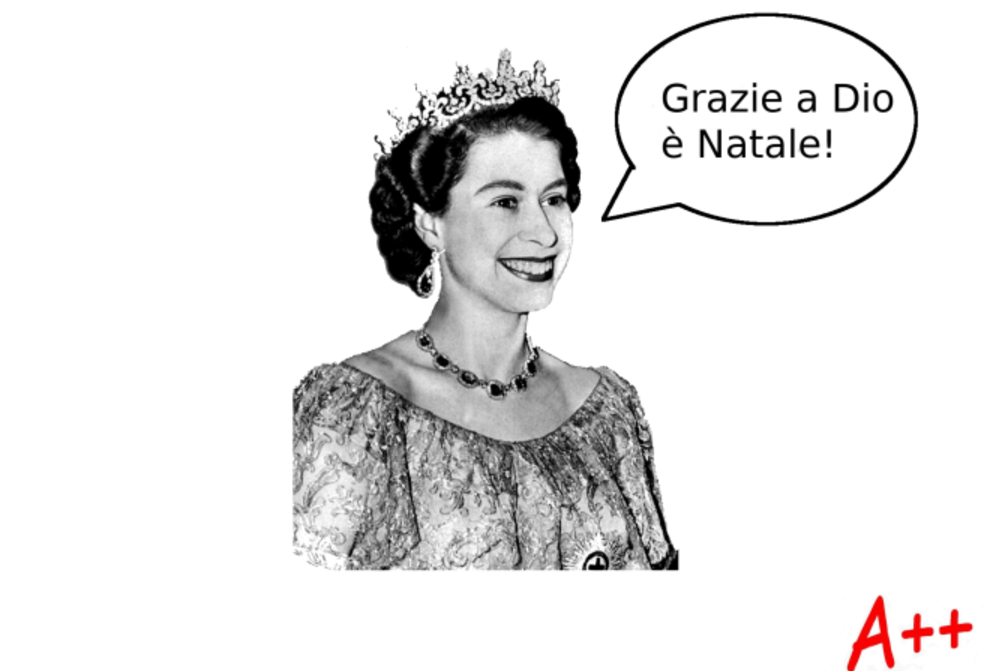
\includegraphics[width=1\columnwidth]{finalqueen.pdf}
\end{figure}
\large{NSTY $\overline{\text{EMMCPP}}$LLLCPP}
\end{center}

\end{document}
